\section{Durchführung}
\label{sec:Durchführung}
In \autoref{fig:RonAuf} ist die Versuchsapperatur zu sehen. Es wurde hier eine Kupfer-Röntgenröhre und als Gitter ein LiF-Kristall
und ein Plexiglas-Streuer verwendet. Der verwendete Aufbau kann manuell oder per PC gesteuert werden. Für diesen Versuch wird
eine Beschleunigungsspannung von $\SI{35}{\kilo\volt}$ und ein Emissionsstrom von $\SI{1}{\milli\ampere}$ eingestellt.
Auf der integrierten Anzeige des Gerätes kann dann die Zählrate abgelesen werden.
\begin{figure}[H]
    \centering
    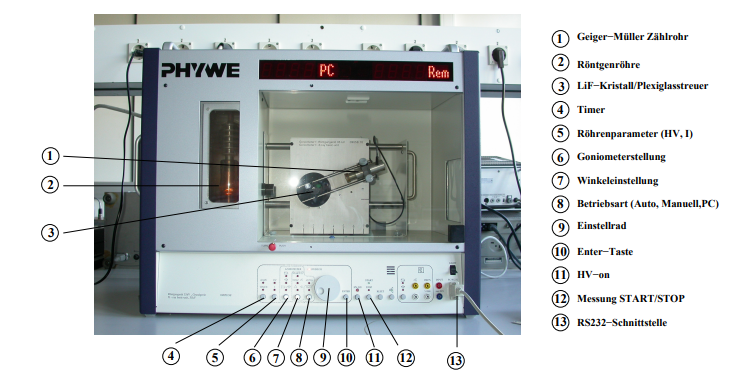
\includegraphics[scale=1]{content/RontgenAufbau.png}
    \caption{Die verwendete Versuchsapperatur mit den einzelnen Komponenten.\cite{sample}}
    \label{fig:RonAuf}
\end{figure}

\subsection{Aufnahme des Emissionsspektrums}
Zur aufnahme des Emissionsspektrums von Kupfer wurde eine $\SI{2}{\milli\meter}$ Blende und ein LiF-Kristall verwendet.
Es wurde das Röntgenspektrum digital in $\symup{\Delta}\alpha=\SI{0,1}{\degree}$-Schritten mit einer Integrationszeit $t = \SI{10}{\second}$ gemessen.
Der Winkel lag dabei zwischen $\SI{8}{\degree} \leq \alpha \leq \SI{25}{\degree}$.

\subsection{Bestimmung der Transmisson als Funktion der Wellenlänge}
Um die Transmisson als Funktion der Wellenlängen zu bestimmen wurde in Schritten von $\symup{\Delta}\alpha=\SI{0,1}{\degree}$ und
einer Integrationszeit $t = \SI{200}{\second}$ die Zählrate der Röntgenstrahlung in einem Winkelbereich
von $\SI{7}{\degree}\leq \alpha \leq \SI{10}{\degree}$ gemessen. Dabei wurde einmal mit Aluminium-Absorber($N_{Al}$)
und einmal ohne($N_0$) digital gemessen. Dafür wurde einmal der Aluminium-Absorber vor die $\SI{2}{\milli\meter}$ Blende gesetzt.

\subsection{Bestimmung der Compton-Wellenlänge}
Für die Bestimmung der Compton-Wellenlänge wurde die $\SI{2}{\milli\meter}$ Blende mit der $\SI{5}{\milli\meter}$ Blende und
der LiF-Kristall durch einen Plexiglas-Streuer ersetzt. Die Integrationszeit betrug dabei $t = \SI{300}{\second}$ und der Kristall
wurde auf $\SI{45}{\degree}$ eingestellt, sowie das Geiger-Müller-Zählrohr auf $\SI{90}{\degree}$.
Es wurde \autoref{fig:Messung} entsprechend die Intensitäten $I_0$, $I_1$ und $I_2$ gemessen.
Dabei befand sich bei der Messung von $I_0$ kein Aluminium-Absorber in der Apperatur. Dieser wurde zur Messung von $I_1$
zwischen die Röntgenröhre und den Streuer gesetzt und anschließend zur Messung von $I_2$ zwischen Streuer und
Geiger-Müller-Zählrohr verbaut. Die Messungen der Intensitäten wurden fünf Mal wiederholt.
\begin{figure}[H]
    \centering
    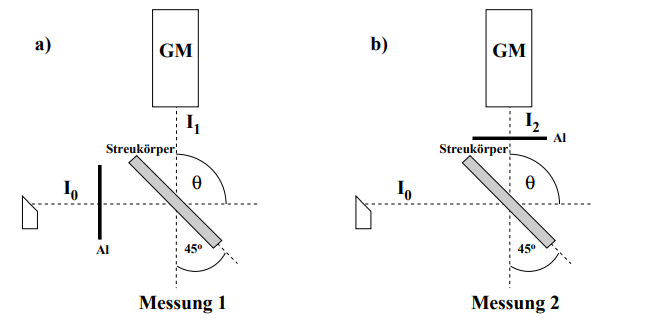
\includegraphics[scale=1]{content/Messung.png}
    \caption{Der Aufbau des Experiments.\cite{sample}}
    \label{fig:Messung}
\end{figure}

\subsection{Aufgaben zur Vorbereitung}
Zur Vorbereitung sollten die Energien der Kupfer $K_\alpha$ und $K_\beta$ Linien recherchiert werden.\cite{Copper}
Diese betragen
\begin{align*}
    K_\alpha &= \SI{8047,78}{\electronvolt}\\
    K_\beta &= \SI{8905,29}{\electronvolt}. 
\end{align*}
Außerdem sollten die zugörigen Wellenlängen und Winkel $\alpha$ berechnet werden.
Nach Gl.\eqref{eqn:EHF} ergibt sich
\begin{align*}
    \lambda_{K_\alpha} &= \SI{15,4060}{\nano\meter}\\
    \lambda_{K_\beta} &= \SI{13,9225}{\nano\meter}
\end{align*}
und damit durch Gl.\eqref{eqn:Bragg} mit $n=1$ und $d = d_{LiF}$
\begin{align*}
    \alpha_{K_\alpha} &= \SI{22,4869}{\degree}\\
    \alpha_{K_\beta} &= \SI{20,2211}{\degree} .
\end{align*}
Zuletzt sollte die Compton-Wellenlängen $\lambda_c$ berechnet werden. Nach $\lambda_c = \frac{h}{m_ec}$ ergibt sich
\begin{equation*}
    \lambda_c = \SI{2,4363}{\pico\meter}.
\end{equation*}
Die verwendeten Konstanten $h$, $c$, $m_e$ und $e$ wurden \cite{Gerth} entnommen.
